\documentclass[twocolumn]{revtex4-2}
\usepackage{graphicx}
\usepackage{amsmath}
\usepackage{hyperref}
\usepackage{xcolor}

\newcommand{\Lagr}{\mathcal{L}}

\begin{document}

\date{\today}
\author{Sixten Nordegren}
\title{Chaos in the double pendulum}

\maketitle

\section{Introduction}
The purpose of this assignment is to find solutions to and solve the double pendulum system. And, beyond that analyze the chaotic behaviour that emerges from it. 
\begin{figure}[b]
	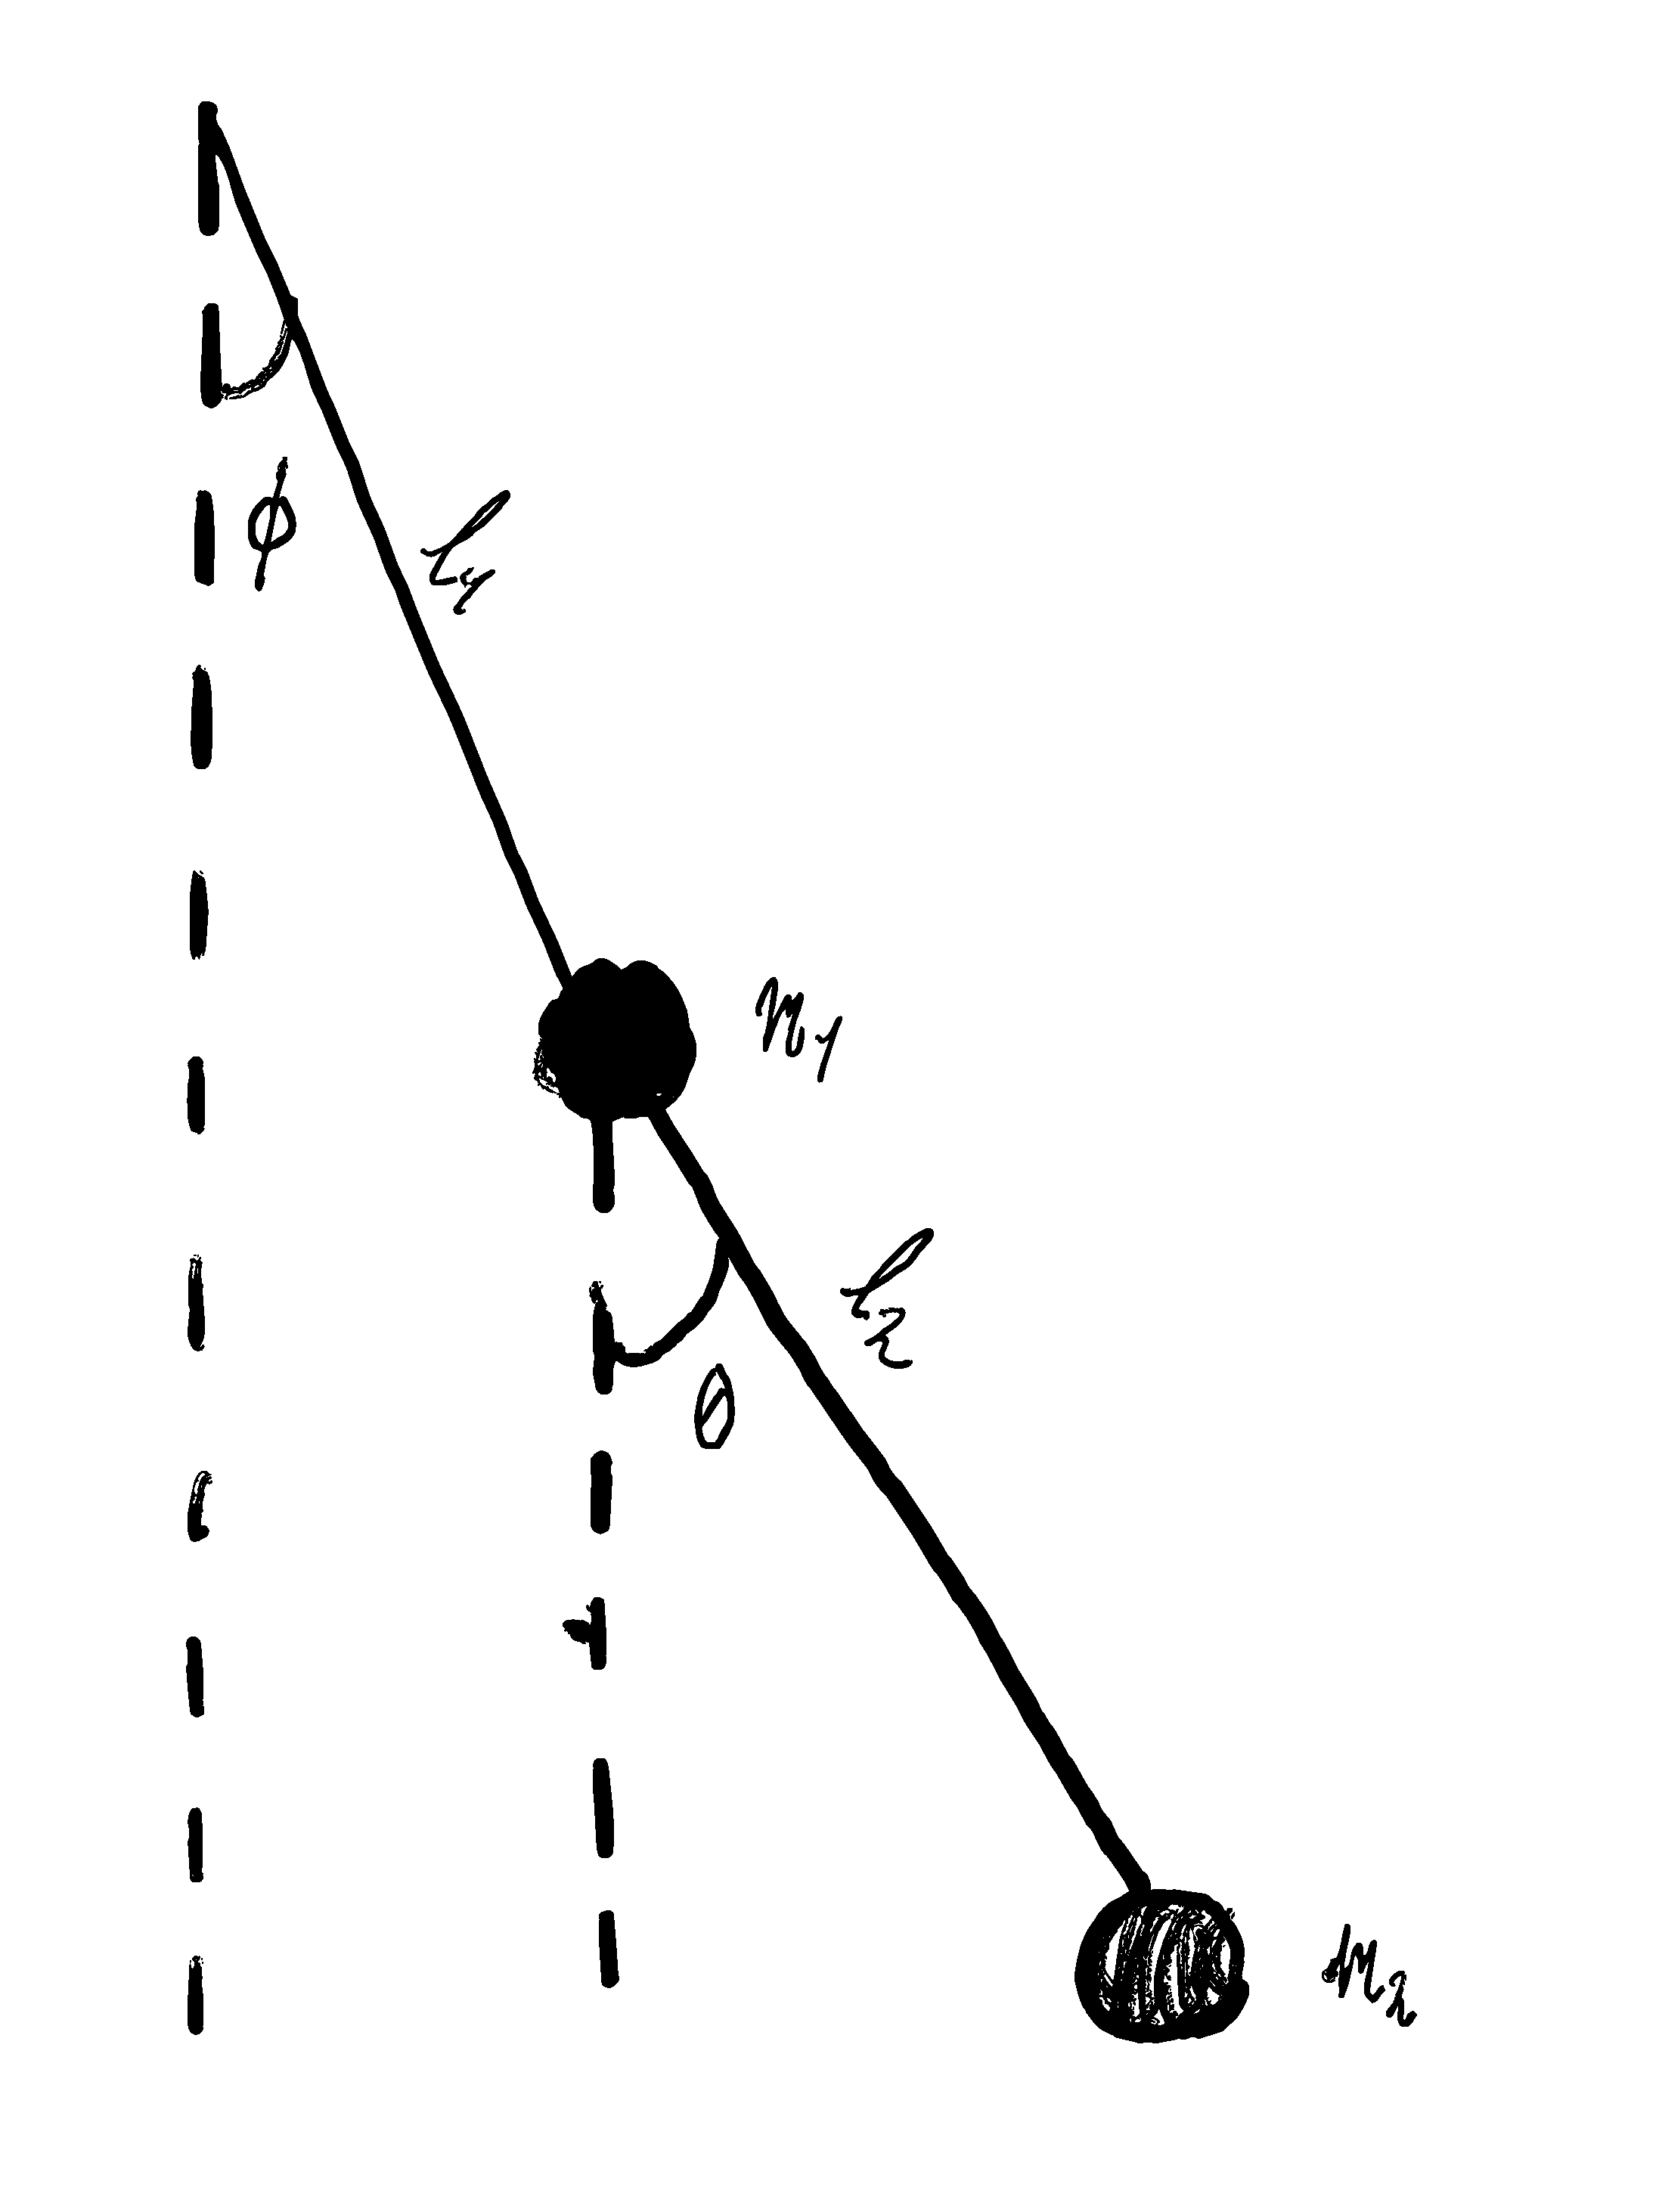
\includegraphics[width=0.5\linewidth]{~/Documents/anme/handin/test.pdf}
	\caption{Doubble pendulum \label{fig: doubble pendulum}}
\end{figure}
\section{Method}
\subsection{Lagrangian approach to the doubble pendulum}
Using the coordinates shown in \ref{fig: doubble pendulum}. We can observe that we have four degrees of freedom with two constraints. This leaves us with $4 - 2  = 2$ generalized coordinates required to describe the system. \footnote{Here we note that since the only conserved quantity is energy, we do in fact have one more degrees of freedom than conserved quantities. Indicative of a chaotic system.}

In the assignment, I took the liberty of assuming that the only objects in the systems that carry any mass is $m_1$ and $m_2$ marked in \ref{fig: doubble pendulum}. This means that the only part of the system that can hold any energy is those masses. I now then proceed to write out the position vectors of those masses.
\begin{align*}
	r_1 &= (l_1 \sin{(\phi)}, l_1 \cos{(\phi)}) \\
	r_2 &= (l_1 \sin{(\phi)} + l_2 \sin{(\theta)}, l_1 \cos{(\phi)} + l_2\cos{(\theta)})
\end{align*}
Now that we have the position vectors we are ready to try and write the Lagrangian $(\Lagr)$.

\begin{equation}
	\Lagr = \frac{1}{2}m\dot r_1^2 + \frac{1}{2}m\dot r_2^2 - V_1 - V_2
	\label{eq: Lagrangian initial}
\end{equation}
\begin{align}
	V_1 &= m_1gl_1(1 - \cos{(\phi)}) \nonumber \\
	V_2 &= m_2g(l_1(1 - \cos{(\phi)}) + l_2(1 - \cos{(\theta)}) )
	\label{eq: init pot}
\end{align}
This expression carries terms that are just constants (If you would to multiply in the factors outside of the parentheses) which later on, in the Euler-Lagrange equations cancell. For this reason, any further refrence to \ref{eq: init pot} will be made without them. \footnote{From what I can tell, this is the standard way of treating the constants to parts of the lagrangian that ends up disapering. Typically, without any reference to doing so whatsoever. Which I personally find very confusing. So I decided to include a small paragraph notifying the reader of doing so.}
\begin{align*}
	\dot r_1^2 &= ( l_1 \dot \phi )^2 \\
	\dot r_2^2 &= l_1^2 \dot \phi ^2 + l_2 \dot \theta ^2 +... \\
		   &  ... + 2l_1l_2(
	\cos{(\phi)}\cos{(\theta)} + \sin{(\phi)}\sin{(\theta)}
	)\dot \phi \dot \theta
\end{align*}
Which turns \ref{eq: Lagrangian initial} into;

\begin{widetext}
	\begin{equation}
		\Lagr = \frac{m_1}{2}l_1 ^2 \dot \phi ^2 + \frac{ m_2 }{2}\left(l_1^2 \dot \phi ^2
		+ l_2^2 \dot \phi ^2 + 2l_1l_2(
	\cos{(\phi)}\cos{(\theta)} + \sin{(\phi)}\sin{(\theta)}
	)\dot \phi \dot \theta
\right) + g(m_1 + m_2)(\cos{(\phi)})l_1 + gm_2l_2(\cos{(\theta)})
	\end{equation}
\end{widetext}
We can shorten this expression slightly by using the identity $ \cos{(s)}\cos{(t)} + \sin{(s)}\sin{(t)}
= \cos{(s - t)}$ But it doesn't get more compact than that.

Now turning to the Euler-Lagrange equations: 
\begin{equation}
	\frac{\partial \Lagr}{\partial q_i} = \frac{d}{dt}\frac{\partial \Lagr}{\partial \dot q_i}
	\label{eq: E-L}
\end{equation}

\begin{align*}
	\frac{\partial \Lagr}{\partial \phi} &= - m_2l_1l_2\dot \phi \dot \theta \sin{(\phi - \theta)} -
	g(m_2+m_1)l_1\sin{(\phi)} \\
	\frac{\partial \Lagr}{\partial \theta} &=  m_2l_1l_2\dot \phi \dot \theta \sin{(\phi - \theta)} -
	gm_2l_1\sin{(\theta)} \\
	\frac{d}{dt}\left(\frac{\partial \Lagr}{\partial \dot \phi} \right) &= l_1^2(m_1 +m_2)\ddot \phi +
	m_2l_1l_2\ddot \theta\cos{(\phi - \theta)}
	 \\
	& \quad ... - m_2l_1l_2\dot \theta \sin{(\phi - \theta)}\dot \phi  + m_2l_1l_2
\dot \theta \dot \phi \sin{(\phi - \theta)} \\
	\frac{d}{dt} \left( \frac{\partial \Lagr}{\partial \dot \theta} \right) &= l_2^2m_2\ddot \theta +
	m_2l_1l_2\ddot \phi\cos{(\phi - \theta)}
	 \\
	& \quad ... - m_2l_1l_2\dot \phi^{2} \sin{(\phi - \theta)}  - m_2l_1l_2
\dot \theta \dot \phi \sin{(\phi - \theta)} \\
\end{align*}

With these expressions we can now write \ref{eq: E-L} as:
\begin{widetext}
	\begin{equation}
 -g(m_2+m_1)l_1\sin{(\phi)} = 
 l_1^2(m_1 +m_2)\ddot \phi +
	m_2l_1l_2\ddot \theta\cos{(\phi - \theta)} + m_2l_1l_2
\dot \theta \dot \phi \sin{(\phi - \theta)} 
	\label{eq: diff 1it 1}
	\end{equation}
	\begin{equation}
- gm_2l_1\sin{(\theta)}  = 
 l_2^2m_2\ddot \theta +
	m_2l_1l_2\ddot \phi\cos{(\phi - \theta)}
	- m_2l_1l_2\dot \phi^{2} \sin{(\phi - \theta)} 
	\label{eq: diff 1it 2}
	\end{equation}
\end{widetext}
These are nothing but a seccond degree differential equation. We could try to solve that but instead, the easier approach is to try and turn it into a first degree differential equation. We can do this by first using equations \ref{eq: diff 1it 1} and \ref{eq: diff 1it 2} as a linear systems of equations and solving for the seccond derrivatives.\textcolor{red}{ I'll show this derrivation in appendix A.} Now defining new coordinates $\omega_1 = \dot \phi$ and $\omega_2 = \dot \theta$ allows us to write the following :
\begin{equation}
	\left(
	\begin{array}{c}
		\dot \phi \\
		\dot \theta \\
		\ddot \phi \\
		\ddot \theta
	\end{array} \right)  =
	\left(\begin{array}{c}
		\omega_1 \\
		\omega_2 \\
		g_1(\phi, \theta, \omega_1, \omega_2) \\
		g_2(\phi, \theta, \omega_1, \omega_2)
	\end{array}\right)
\end{equation}
\footnote{Definitions of $g_1$ and $g_2$ will be included in the appendix}.

\end{document}

